\chapter{Aufzählungen und Tabellen}

Eine normale Punktliste:
\begin{itemize}
\item Lorem ipsum dolor sit amet, consectetuer adipiscing elit. Nulla ac ipsum a metus viverra tempor. 
\item Nunc sem. Nulla nec urna eu nibh vehicula convallis. Integer ac turpis. Donec mauris enim, dignissim quis, scelerisque ac, rhoncus id, sapien. 
\item Donec turpis felis, cursus in, varius vitae, mollis ac, lorem. Integer a dui sit amet eros nonummy aliquet. Donec egestas adipiscing tellus. Nulla iaculis. 
\item Aliquam erat volutpat. Curabitur posuere, eros vitae accumsan semper, risus erat viverra erat, eu vehicula mi leo at elit. Fusce luctus. Fusce vehicula pretium diam. Nunc sed arcu ut erat suscipit fermentum.
\end{itemize}

Eine nummerierte Liste:
\begin{enumerate}
\item Lorem ipsum dolor sit amet, consectetuer adipiscing elit. Nulla ac ipsum a metus viverra tempor. 
\item Nunc sem. Nulla nec urna eu nibh vehicula convallis. Integer ac turpis. Donec mauris enim, dignissim quis, scelerisque ac, rhoncus id, sapien. 
\item Donec turpis felis, cursus in, varius vitae, mollis ac, lorem. Integer a dui sit amet eros nonummy aliquet. Donec egestas adipiscing tellus. Nulla iaculis. 
\item Aliquam erat volutpat. Curabitur posuere, eros vitae accumsan semper, risus erat viverra erat, eu vehicula mi leo at elit. Fusce luctus. Fusce vehicula pretium diam. Nunc sed arcu ut erat suscipit fermentum.
\end{enumerate}

\section{Vom Autor verwendete Software}
\label{sec:Werkzeuge}
Im Folgenden werden die Programme vorgestellt, die der Autor zum Erstellen dieser Arbeit und vor allem zur Entwicklung der Webservices verwendet hat. Soweit es möglich war, wurden Open-Source-Programme eingesetzt.

\begin{itemize}
\itemd{Microsoft Visio}{Die EPKs der BAP wurden mit Microsoft Visio erstellt. Der Autor hat zwar verschiedene Open-Source-Programme\footnote{Dia, OpenOffice Draw und die EPC Tools.} ausprobiert, mit denen EPKs erstellt werden könnten, die grafischen Ergebnisse waren aber nicht zufriedenstellend. Die Symbole von Visio sehen den "`originalen"' ARIS-Symbolen am ähnlichsten und können darüber hinaus mit zusätzlichen Informationen wie Dauer und Kosten versehen werden.}
\itemd{PSPad}{Für die Bearbeitung von verschiedenen (Text-)Dateien wurde der Texteditor PSPad verwendet. Mit diesem konnten \zB auch die regulären Ausdrücke für die XML-Schemas entwickelt werden. Website: \url{http://www.pspad.com/}}
\itemd{Eclipse}{Sowohl der ActiveBPEL Designer als auch die EntireX Workbench sind Plugins für die IDE Eclipse. Auch zur Java- und PHP-Entwicklung wurde dieses Werkzeug verwendet. Website: \url{http://www.eclipse.org/}}
\itemd{XML Copy Editor}{Für die Entwicklung der XML-Schemas und die Bearbeitung von XML-Dateien wurde der XML Copy Editor eingesetzt. Mit diesem können \ua XML-Dateien auf Wohlgeformtheit geprüft und gegen ihr Schema validiert werden. Website: \url{http://xml-copy-editor.sourceforge.net/}}
\itemd{soapUI}{
Mit soapUI können Webservices getestet werden, ohne einen Client zu programmieren. Die SOAP-Anfragen werden automatisch anhand der WSDL generiert und die Antworten können gegen die WSDL-Datei validiert werden. Website: \url{http://www.soapui.org/}}
\itemd{Ethereal}{
Die Netzwerkkommunikation beim Aufrufen der Webservices wurde mit Ethereal, einem umfangreichen Werkzeug zur Analyse des Netzwerkverkehrs, mitgeschnitten. Website: \url{http://www.ethereal.com/}}
\itemd{\LaTeX}{
Diese Arbeit wurde mit {\LaTeX} geschrieben. Als Distribution wurde MiKTeX verwendet und als Editor der LaTeX Editor. Websites: \url{http://miktex.org/}, \url{http://www.latexeditor.org/}}
\end{itemize}

\section{Elemente der Ereignisgesteuerten Prozesskette}

\begin{longtable}{|m{10cm}|m{3cm}|}
\caption{Elemente der Ereignisgesteuerten Prozesskette} \\
\hline
\label{tab:ElementeDerEreignisgesteuertenProzesskette}
\textbf{Element} & \textbf{Symbol}\\
\hline
\textbf{Funktion} 

Funktionen beschreiben Tätigkeiten, die im Verlauf des Geschäftsprozesses anfallen. Sie können von Mitarbeitern oder einem Informationssystem durchgeführt werden und benötigen evtl. Ressourcen, die ihnen zugewiesen werden. 

Beispiele: \textit{Auftrag anlegen}, \textit{Rechnung schreiben}, \textit{Konto abschließen} & 
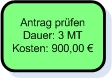
\includegraphics[width=3cm]{EPK-Funktion.jpg} \\
\hline
\textbf{Ereignis} 

Ereignisse sind betriebswirtschaftlich relevante Ereignisse, die den Geschäftsprozess in irgendeiner Weise steuern oder beeinflussen. Ereignisse sind immer Auslöser oder Ergebnisse von Funktionen. Ein Geschäftsprozess beginnt und endet stets mit einem Ereignis. 

Beispiele: \textit{Auftrag eingetroffen}, \textit{Überweisung getätigt}, \textit{Rechnung erstellt} & 
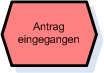
\includegraphics[width=3cm]{EPK-Ereignis.jpg} \\
\hline
\textbf{Operatoren} 

Operatoren steuern den Kontrollfluss eines Geschäftsprozesses. Sie machen \zB deutlich, dass eine Funktion mehrere Ereignisse auslöst, oder zeigen alternative Vorgehensweisen an. Es gibt drei Operatoren (v.\,l.\,n.\,r.\,): UND, ODER und XODER (exklusives ODER). & 

\includegraphics[width=3cm]{EPK-Operatoren.jpg} \\
\hline
\textbf{Organisationseinheit} 

Organisationseinheiten werden Funktionen zugeordnet und beschreiben, wo die Funktionen ausgeführt werden bzw. wer sie ausführt. Die Bezeichnung der Symbole enthält zusätzlich zur Abteilung noch die Namen der Mitarbeiter.

Beispiele: \textit{Vertrieb}, \textit{Personal}, \textit{Produktion} & 
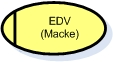
\includegraphics[width=3cm]{EPK-Organisationseinheit.jpg} \\
\hline
\textbf{Informationsobjekt} 

Auch Informationsobjekte werden Funktionen zugewiesen und beschreiben die von diesen benötigten oder erstellten Informationen. Dabei sind sämtliche Formen von Informationen auf verschiedenen Datenträgern möglich und nicht etwa nur digitale Daten. Die Bezeichnung der Symbole enthält zusätzlich das Informationssystem, aus dem die Informationen stammen.

Beispiele: \textit{Kundendatenbank}, \textit{Versicherungsantrag}, \textit{Rechnung} & 
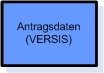
\includegraphics[width=3cm]{EPK-Informationen.jpg} \\
\hline
\textbf{Prozesswegweiser}

Mit Prozesswegweisern werden Prozesse, die in anderen EPKs beschrieben sind, referenziert. So können \zB unübersichtliche Prozesse in Teilprozesse gegliedert und häufig verwendete Prozesse an zentraler Stelle modelliert werden. Prozesswegweiser stehen in einer EPK immer anstelle von Funktionen. & 
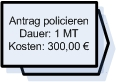
\includegraphics[width=3cm]{EPK-Prozesspfad.jpg} \\
\hline
\end{longtable}
